\chapter{Integer Programming and Graphs}
In this chapter we introduce the concept of Integer programming. We will approach the subject with examples and results from graph theory, but apart from fundamental definitions we will omit most of the theory from this field of mathematics. A more in depth explanation can be found in ~\cite{wolsey1998integer}. 
\section{Some graph notation}
\begin{definition}\label{graph}
A \textbf{graph} $G$ is a pair $(V,E)$ where $V$ is a set of vertices and $E$ is a set of edges and each edge in $E$ is a subset of $V$ containing two vertices.
\end{definition}
\begin{definition}
Let $G=(V,E)$ be a graph. Two vertices $v,u\in V$ are said to be \textbf{adjacent} if the edge $(v,u)$ (or $(u,v)$) is in $E$.
\end{definition}
\begin{definition}
Let $G=(V,E)$ be a graph. A subset $S$ of $V$ forms an \textbf{independent set} if no two vertices in $S$ are adjacent in $G$.
\end{definition}
\begin{definition}
Let $G=(V,E)$ be a graph. A subset $S$ of $V$ forms a \textbf{clique} if all pairs of two vertices in $S$ are adjacent in $G$.
\end{definition}
\begin{definition}
Let $G=(V,E)$ be a graph. A \textbf{maximal independent set} or a \textbf{maximal clique} is an independent set or a clique respectively where if any other vertex $v \in V$ is added to the set, it will lose the property of being an independent set or clique respectively.
\end{definition}
\begin{definition}
A \textbf{maximum independent set} or a \textbf{maximum clique} in a graph $G$ is an independent set or a clique respectively where no other independent set or clique in $G$ respectively have more vertices.
\end{definition}
\begin{definition}
The \textbf{clique number} $\omega(G)$ of a graph $G$ is the number of vertices in a maximum clique in $G$.
\end{definition}

\section{Mixed Integer Programming - MIP}
A Mixed integer problem (MIP) is a way of formulating optimization problems with integer values. The structure of an integer problem is the same as of a linear problem, but with the extra constraint that all or some of the variables are in $\Z$. This added constraint might seem insignificant, but it introduces crucial differences compared to purely linear problems. One significant difference is that the feasible space of an MIP consists of disjoint sets with no feasible solutions between the integer values of the integer variables and thus it is not convex.
\begin{figure}[H]\label{IP figure}
\centering
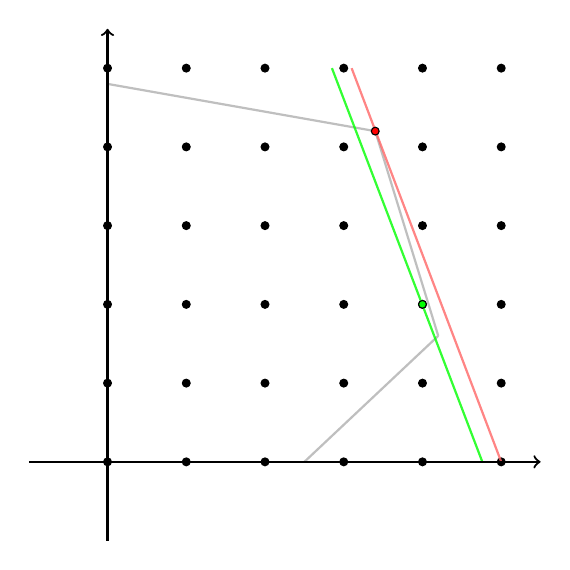
\begin{tikzpicture}
\foreach \x in {0,...,5}{
	\foreach \y in {0,...,5}{% node on the grid we have drawn 
        \node[draw,circle,inner sep=1pt,fill] at (\x,\y) {};
            % Places a dot at those points
  }
}
\draw [lightgray, thick] (0,4.8) -- (3.4,4.2);
\draw [lightgray, thick] (3.4,4.2)--(4.2,1.6);
\draw [lightgray, thick] (4.2,1.6)--(2.5,0);
\draw [red!60,opacity=.8, thick] (3.1,5)--(5,0);
\node[draw,circle,inner sep=1pt,fill = red] at (3.4,4.2) {};
\draw [green,opacity=.8, thick] (2.85,5)--(4.76,0);
\node[draw,circle,inner sep=1pt,fill = green] at (4,2) {};
\draw [black, thick, arrows = ->] (0,-1) -- (0,5.5);
\draw [black, thick, arrows = ->] (-1,0) -- (5.5,0);
\end{tikzpicture}
\caption{Figure showing the feasible region of an IP with the optimal solution in green and the optimal solution to the linear relaxation in red (see \Cref{relaxation})}
\end{figure}
\begin{example}
In the case of \Cref{lpex} the optimal solution did not have integer values, but when buying food it's often only possible to buy a product in quantities of natural numbers. If we restrict $x_2$ to be an integer we will get a new optimal solution, $x_1=0.75, x_2=2$ and $x_3= 3.5$ with an objective value of 12.75, and if we restrict all variables to be integral, an optimal solution would be $x_1=1, x_2=2$ and $x_3= 3$ with the objective value 13.\\
These solutions are fairly close to the solution to the LP, but as seen in \Cref{IP figure} we can't always expect this to be the case for MIPs.
\end{example}
\subsection{Integer and Binary Constraints}
An important method in Integer programming is \textbf{Binary programming}. Here variables take values either $1$ or $0$. These binary variables are very useful since they can easily be used to say "If variable $x_i$ is part of the solution then $x_i = 1$ otherwise $x_i = 0$". Binary constraints will be used extensively once we start colouring graphs. We begin with an easier combinatorial problem on graphs using an MIP formulation:
\begin{example}\label{independent set}
Maximum clique and maximum independent set problem:\\
Let $G=(V,E)$ be a graph and let $H=(V,E')$ with $E' = \{(u,v):u,v\in V, (u,v) \notin E\}$ be it's complement graph. Then
\begin{align}
\begin{array}{ll@{}ll}
\text{max} &\sum_{v\in V} x_v&\\
\text{s.t.} &x_u + x_v \leq 1,& \forall (u,v) \in E\\
&x_v\in\{0,1\},& \forall v \in V\\
\end{array}
\end{align}
calculates the maximum independent set and
\begin{align}
\begin{array}{ll@{}ll}
\text{max} &\sum_{v\in V} x_v&\\
\text{s.t.} &x_u + x_v \leq 1,& \forall (u,v) \in E'\\
&x_v\in\{0,1\},& \forall v \in V\\
\end{array}
\end{align}
calculates the maximum clique.
% Clique and independent set
\begin{figure}[H]
\centering
\begin{tikzpicture}[main node/.style={circle,fill=blue!20,draw,minimum size=.8cm,inner sep=0pt}]
    \node[main node,fill = green!60] (1) {$v_1$};
    \node[main node] (2) [right = 1.5cm  of 1]  {$v_2$};
    \node[main node] (3) [below left = 1cm and .8cm of 1] {$v_3$};
    \node[main node,fill = green!60] (4) [below right = 1cm and .8cm of 2] {$v_4$};
    \node[main node] (5) [below = 2.4cm  of 1] {$v_5$};
    \node[main node,fill = green!60] (6) [right = 1.5cm  of 5] {$v_6$};
    \node[left = 1cm of 1]{$G:$};

    \path[draw,thick]
    (1) edge node {} (2)
    (1) edge node {} (3)
    (1) edge node {} (5)
    (2) edge node {} (3)
    (2) edge node {} (4)
    (2) edge node {} (5)
    (3) edge node {} (4)
    (3) edge node {} (6)
    (4) edge node {} (5)
    (5) edge node {} (6)
    ;
    \begin{scope}[xshift=6cm]
    \node[main node] (1) {$v_1$};
    \node[main node,fill = green!60] (2) [right = 1.5cm  of 1]  {$v_2$};
    \node[main node,fill = green!60] (3) [below left = 1cm and .8cm of 1] {$v_3$};
    \node[main node,fill = green!60] (4) [below right = 1cm and .8cm of 2] {$v_4$};
    \node[main node] (5) [below = 2.4cm  of 1] {$v_5$};
    \node[main node] (6) [right = 1.5cm  of 5] {$v_6$};
    \node[left = 1cm of 1]{$G:$};

    \path[draw = gray,thick]
    (1) edge node {} (2)
    (1) edge node {} (3)
    (1) edge node {} (5)
    (2) edge node {} (3)
    (2) edge node {} (4)
    (2) edge node {} (5)
    (3) edge node {} (4)
    (3) edge node {} (6)
    (4) edge node {} (5)
    (5) edge node {} (6);
    %%
    \path[draw=red,thick,dashed]
    (1) edge node {} (4)
    (1) edge node {} (6)
    (2) edge node {} (6)
    (3) edge node {} (5)
    (4) edge node {} (6)
    ;
    \end{scope}
\end{tikzpicture}
\caption{Shown in green is a maximum independent set and a maximum clique in a graph $G$.}
\end{figure}
\begin{proof}
We need to prove two implications: An optimal solution to the MIP is an optimal solution to the problem, and an optimal solution to the problem is an optimal solution to the MIP. 

An optimal solution to the independent set MIP forms a maximum independent set in $G=(V,E)$ consisting of the vertices $\{v\in V:x_v=1\}$:
\begin{enumerate}
\item The first constraint states that no two adjacent vertices can be in the solution simultaneously. Thus a feasible solution forms an independent set.
When maximizing $\sum_{v\in V} x_v$ an optimal solution will form an independent set with the biggest number of vertices possible. Thus an optimal solution forms a maximal independent set in $G$
\end{enumerate}
A maximum independent set $I\subset V$, with values $x_v$ defined as $$x_{v} = \left\{
\begin{array}{ll}
1 & \text{if } v \in I \\ 0 & \text{otherwise}
\end{array}\right.$$ is an optimal solution to the MIP:
\begin{enumerate}
\item Since no vertices in $I$ are connected by an edge by definition, the solution is feasible. The objective value of this solution is exactly the number of vertices in the maximum independent set, and since $I$ is maximum the solution is optimal.
\end{enumerate}

\noindent In the maximum clique problem any two adjacent vertices in the component graph $H$ indicates that they are not adjacent in the $G$ and any two adjacent vertices in $G$ are independent of each other in $H$. Then it follows that an independent set in $H$ are all adjacent in $G$ and form a clique. \\
The rest of the proof follows from the proof of the maximal independent set formulation.
\end{proof}
\end{example}
\section{Relaxation}\label{relaxation}
It is well known that \ref{independent set} is an $\mathcal{NP}$-hard problem. Thus unlike Linear programming, with real variables, integer programming can be used to solve $\mathcal{NP}$-hard problems. In some cases it is however still useful to view the IP as a linear problem and assign real values to the variables instead of integer. This problem, where values in $\Z$ are assigned values in $\R$ instead and binary variables are assigned values in $[0,1]$ is called the \textbf{linear relaxation} of the IP. And the solution to the linear relaxation of an IP can often tell us something about the solution to the IP itself or even give the integer solution.
\begin{example}
Some examples of cases where the relaxation is useful to different degrees are the following formulations of the shortest path problem and the shortest cycle problem in graphs together with the formulation of the maximal independent sets problem \ref{independent set}.
\section{Length of shortest path between two vertices}
Let $G=(V,E)$ be a directed graph where $V$ is the set of vertices and $E$ is the set of edges. Let $A$ be the adjacency matrix of $G$ and introduce the set of binary values $x_{i,j}$ where
\begin{align*}
x_{i,j} = \left\{
\begin{array}{ll}
1 & \text{if } (i,j) \text{ is in the path} \\ 0 & \text{otherwise}
\end{array}\right.
\end{align*}
And the sets $V^+(i)$ and $V^-(i)$ where
\begin{align*}
V^+(i) = \{v: (i,v) \in E\}\\
V^-(i) = \{v: (v, i) \in E\}
\end{align*}
We want to minimize $\sum x_{i,j}$ subject to conditions that ensures we get a path form $s \in V$ to $t \in V$ in $G$.
\begin{align}
\begin{array}{ll@{}ll}
\text{min} &\sum_{i,j \in V}x_{i,j}&\\
\text{s.t.} &\sum_{j\in V^+(s)}x_{s,j} = 1,&\\
&\sum_{i\in V^-(t)}x_{i,t} = 1,&\\
&\sum_{j\in V^+(v)}x_{v,j} = \sum_{i\in V^-(v)}x_{i,v}, \quad &\forall v \in V \backslash \{s,t\},\\
&x_{i,j}\leq A_{i,j},&\forall i,j \in V,\\
&x_{i,j} \in \{0,1\},&\forall i,j \in V.\\
\end{array}
\end{align}
In this case the convex hull of the feasible set has all its extreme points in integer points. Thus the relaxed problem with $x_{i,j} \in [0,1]$ has has optimal solutions in integral values and we don't have to solve the original IP at all.\\
This is not surprising because there are obvious poly-time algorithms for this problem.
\section{Length of shortest directed cycle in a graph}
Let $G=(V,E)$ be a directed graph where $V$ is the set of vertices and $E$ is the set of edges. Let $A$ be the adjacency matrix of $G$ and introduce the set of binary values $x_{i,j}$ where
\begin{align*}
x_{i,j} = \left\{
\begin{array}{ll}
1 & \text{if } (i,j) \text{ is in the cycle} \\ 0 & \text{otherwise}
\end{array}\right.
\end{align*}
We want to minimize $\sum x_{i,j}$ subject to conditions that ensures we get a cycle in $G$.
\begin{align}
\begin{array}{ll@{}ll}
\text{min} & \sum_{i,j \in V}x_{i,j}&\\
\text{s.t.} & \sum_{j\in V}x_{i_0,j} = \sum_{i\in V}x_{i,j_0},& \forall j_0,i_0 \in V,\\
&x_{i,j}\leq A_{i,j} \leq 1,&\forall i,j \in V,\\
&\sum_{i,j\in V}x_{v,j} \geq 1&\\
&x_{i,j} \in \{0,1\},&\forall i,j \in V.\\
\end{array}
\end{align}
In this case a solution to the relaxed problem with $x_{i,j} \in [0,1]$ will be a union of directed cycles and the objective value will always minimize to $1$. Thus the relaxed problem does not tell us much about the actual optimal integral solution, but at least it respects the structure of the problem in some sense.\\
\section{Maximum clique and independent set problem}
In the case of \Cref{independent set} the relaxed problem doesn't tell us much at all. In some cases the relaxed problem will have the same solution as the IP but a solution with $x_v = \frac{1}{2} \text{for all } v \in V$ is always feasible and in most cases it will have a much higher objective value compared to an optimal solution to the MIP. Thus all we can get from the relaxation is a completely trivial upper bound of the actual problem.
\begin{figure}[H]
\centering
\begin{tikzpicture}[main node/.style={circle,fill=blue!20!green!40,draw,minimum size=.8cm,inner sep=0pt}]
    \node[main node] (1) {$x_1=\frac{1}{2}$};
    \node[main node] (2) [right = 1.5cm  of 1]  {$x_2=\frac{1}{2}$};
    \node[main node] (3) [below left = 1cm and .8cm of 1] {$x_3=\frac{1}{2}$};
    \node[main node] (4) [below right = 1cm and .8cm of 2] {$x_4=\frac{1}{2}$};
    \node[main node] (5) [below = 2.4cm  of 1] {$x_5=\frac{1}{2}$};
    \node[main node] (6) [right = 1.5cm  of 5] {$x_6=\frac{1}{2}$};
    \node[left = 1cm of 1]{$G:$};
    \node[below right = -0.1cm and .5cm of 4,fill=blue!20]{\begin{tabular}{l} $\sum_{v\in V} x_v=3$. \\\\ Vertices in max inde-\\ pendend set of $G:1$.\end{tabular}};

    \path[draw,thick]
    (1) edge node {} (2)
    (1) edge node {} (3)
    (1) edge node {} (4)
    (1) edge node {} (5)
    (1) edge node {} (6)
    (2) edge node {} (3)
    (2) edge node {} (4)
    (2) edge node {} (5)
    (2) edge node {} (6)
    (3) edge node {} (4)
    (3) edge node {} (5)
    (3) edge node {} (6)
    (4) edge node {} (5)
    (4) edge node {} (6)
    (5) edge node {} (6)
    ;
\end{tikzpicture}
\caption{An example of how the relaxation of \Cref{independent set} fails to give us information on a graph's maximal independent sets.}
\end{figure}
\end{example}
